% TODO translation
% TODO proof-reading
\subsection{Second example}

Now another simple crackme example:

\begin{lstlisting}
public class password
{
	public static void main(String[] args)
	{
		System.out.println("Please enter the password");
		String input = System.console().readLine();
		if (input.equals("secret"))
			System.out.println("password is correct");
		else
			System.out.println("password is not correct");
	}
}
\end{lstlisting}

Let's load it to IDA:

\begin{figure}[H]
\centering
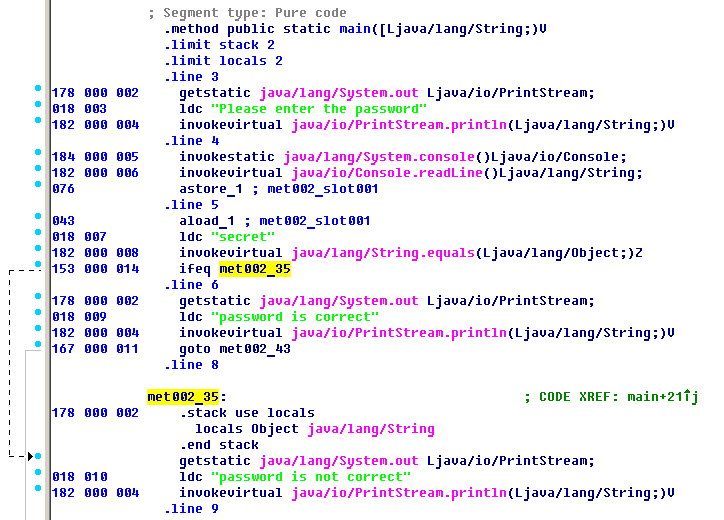
\includegraphics[scale=\FigScale]{Java_and_NET/java/13_patching/2/1.png}
\caption{IDA}
\end{figure}

We see here \TT{ifeq} instruction which do the job.
It means \IT{if equal}, and this is misnomer, I would name it \TT{ifz} (\IT{if zero}), i.e, 
if value at \ac{TOS} is zero, then do the jump.
In our example, it jumps if password is not correct (\TT{equals} method return \TT{False}, which is 0).
The very first idea is to patch it.
There are two bytes in \TT{ifeq} opcode, which encodes jump offset.
To make this instruction idle, we must set byte 3 at 3rd opcode
(because 3 will be added to the current address resulting always jump to the next instruction,
\TT{ifeq} instruction length is 3 bytes):

\begin{figure}[H]
\centering
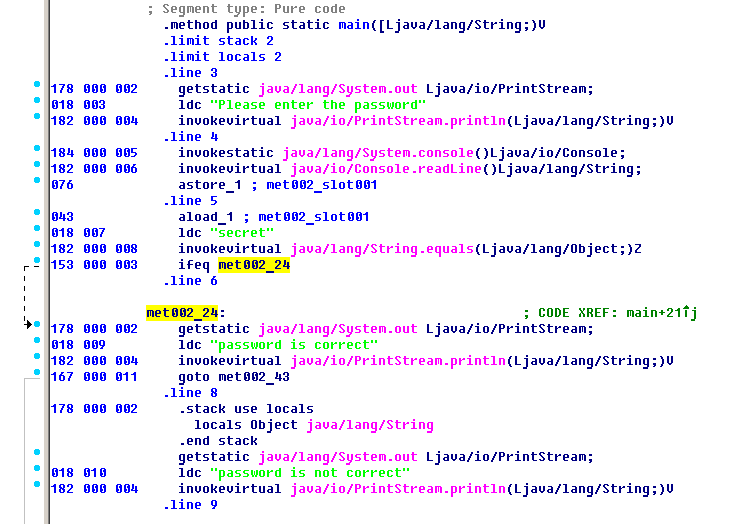
\includegraphics[scale=\FigScale]{Java_and_NET/java/13_patching/2/2.png}
\caption{IDA}
\end{figure}

That doesn't work (JRE 1.7):

\begin{lstlisting}
Exception in thread "main" java.lang.VerifyError: Expecting a stackmap frame at branch target 24
Exception Details:
  Location:
    password.main([Ljava/lang/String;)V @21: ifeq
  Reason:
    Expected stackmap frame at this location.
  Bytecode:
    0000000: b200 0212 03b6 0004 b800 05b6 0006 4c2b
    0000010: 1207 b600 0899 0003 b200 0212 09b6 0004
    0000020: a700 0bb2 0002 120a b600 04b1
  Stackmap Table:
    append_frame(@35,Object[#20])
    same_frame(@43)

        at java.lang.Class.getDeclaredMethods0(Native Method)
        at java.lang.Class.privateGetDeclaredMethods(Class.java:2615)
        at java.lang.Class.getMethod0(Class.java:2856)
        at java.lang.Class.getMethod(Class.java:1668)
        at sun.launcher.LauncherHelper.getMainMethod(LauncherHelper.java:494)
        at sun.launcher.LauncherHelper.checkAndLoadMain(LauncherHelper.java:486)
\end{lstlisting}

But needless to say, it was worked in JRE 1.6.

I also tried to replace all 3 \TT{ifeq} opcodes by zero bytes (\ac{NOP}), 
and it's still doesn't work.
Well, probably there are more stack map checks appeared in JRE 1.7 .

OK, I'll replace the whole call to \TT{equals} method by \TT{iconst\_1} instruction 
plus pack of \ac{NOP}s:

\begin{figure}[H]
\centering
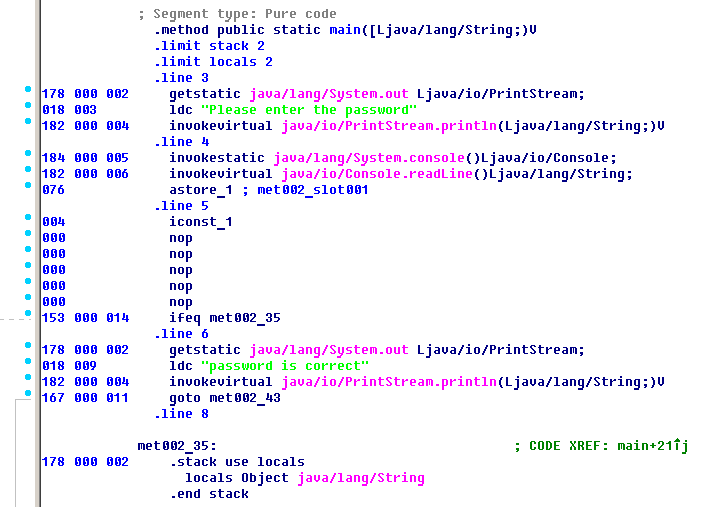
\includegraphics[scale=\FigScale]{Java_and_NET/java/13_patching/2/3.png}
\caption{IDA}
\end{figure}

1 will always be at the \ac{TOP} when \TT{ifeq} instruction will be executed, 
so \TT{ifeq} will never jump.
